% Options for packages loaded elsewhere
\PassOptionsToPackage{unicode}{hyperref}
\PassOptionsToPackage{hyphens}{url}
%
\documentclass[
]{book}
\title{Học xác suất thống kê qua phần mềm R}
\author{Tan Duc Nguyen (aka Duc)}
\date{2022-03-09}

\usepackage{amsmath,amssymb}
\usepackage{lmodern}
\usepackage{iftex}
\ifPDFTeX
  \usepackage[T1]{fontenc}
  \usepackage[utf8]{inputenc}
  \usepackage{textcomp} % provide euro and other symbols
\else % if luatex or xetex
  \usepackage{unicode-math}
  \defaultfontfeatures{Scale=MatchLowercase}
  \defaultfontfeatures[\rmfamily]{Ligatures=TeX,Scale=1}
\fi
% Use upquote if available, for straight quotes in verbatim environments
\IfFileExists{upquote.sty}{\usepackage{upquote}}{}
\IfFileExists{microtype.sty}{% use microtype if available
  \usepackage[]{microtype}
  \UseMicrotypeSet[protrusion]{basicmath} % disable protrusion for tt fonts
}{}
\makeatletter
\@ifundefined{KOMAClassName}{% if non-KOMA class
  \IfFileExists{parskip.sty}{%
    \usepackage{parskip}
  }{% else
    \setlength{\parindent}{0pt}
    \setlength{\parskip}{6pt plus 2pt minus 1pt}}
}{% if KOMA class
  \KOMAoptions{parskip=half}}
\makeatother
\usepackage{xcolor}
\IfFileExists{xurl.sty}{\usepackage{xurl}}{} % add URL line breaks if available
\IfFileExists{bookmark.sty}{\usepackage{bookmark}}{\usepackage{hyperref}}
\hypersetup{
  pdftitle={Học xác suất thống kê qua phần mềm R},
  pdfauthor={Tan Duc Nguyen (aka Duc)},
  hidelinks,
  pdfcreator={LaTeX via pandoc}}
\urlstyle{same} % disable monospaced font for URLs
\usepackage{color}
\usepackage{fancyvrb}
\newcommand{\VerbBar}{|}
\newcommand{\VERB}{\Verb[commandchars=\\\{\}]}
\DefineVerbatimEnvironment{Highlighting}{Verbatim}{commandchars=\\\{\}}
% Add ',fontsize=\small' for more characters per line
\usepackage{framed}
\definecolor{shadecolor}{RGB}{248,248,248}
\newenvironment{Shaded}{\begin{snugshade}}{\end{snugshade}}
\newcommand{\AlertTok}[1]{\textcolor[rgb]{0.94,0.16,0.16}{#1}}
\newcommand{\AnnotationTok}[1]{\textcolor[rgb]{0.56,0.35,0.01}{\textbf{\textit{#1}}}}
\newcommand{\AttributeTok}[1]{\textcolor[rgb]{0.77,0.63,0.00}{#1}}
\newcommand{\BaseNTok}[1]{\textcolor[rgb]{0.00,0.00,0.81}{#1}}
\newcommand{\BuiltInTok}[1]{#1}
\newcommand{\CharTok}[1]{\textcolor[rgb]{0.31,0.60,0.02}{#1}}
\newcommand{\CommentTok}[1]{\textcolor[rgb]{0.56,0.35,0.01}{\textit{#1}}}
\newcommand{\CommentVarTok}[1]{\textcolor[rgb]{0.56,0.35,0.01}{\textbf{\textit{#1}}}}
\newcommand{\ConstantTok}[1]{\textcolor[rgb]{0.00,0.00,0.00}{#1}}
\newcommand{\ControlFlowTok}[1]{\textcolor[rgb]{0.13,0.29,0.53}{\textbf{#1}}}
\newcommand{\DataTypeTok}[1]{\textcolor[rgb]{0.13,0.29,0.53}{#1}}
\newcommand{\DecValTok}[1]{\textcolor[rgb]{0.00,0.00,0.81}{#1}}
\newcommand{\DocumentationTok}[1]{\textcolor[rgb]{0.56,0.35,0.01}{\textbf{\textit{#1}}}}
\newcommand{\ErrorTok}[1]{\textcolor[rgb]{0.64,0.00,0.00}{\textbf{#1}}}
\newcommand{\ExtensionTok}[1]{#1}
\newcommand{\FloatTok}[1]{\textcolor[rgb]{0.00,0.00,0.81}{#1}}
\newcommand{\FunctionTok}[1]{\textcolor[rgb]{0.00,0.00,0.00}{#1}}
\newcommand{\ImportTok}[1]{#1}
\newcommand{\InformationTok}[1]{\textcolor[rgb]{0.56,0.35,0.01}{\textbf{\textit{#1}}}}
\newcommand{\KeywordTok}[1]{\textcolor[rgb]{0.13,0.29,0.53}{\textbf{#1}}}
\newcommand{\NormalTok}[1]{#1}
\newcommand{\OperatorTok}[1]{\textcolor[rgb]{0.81,0.36,0.00}{\textbf{#1}}}
\newcommand{\OtherTok}[1]{\textcolor[rgb]{0.56,0.35,0.01}{#1}}
\newcommand{\PreprocessorTok}[1]{\textcolor[rgb]{0.56,0.35,0.01}{\textit{#1}}}
\newcommand{\RegionMarkerTok}[1]{#1}
\newcommand{\SpecialCharTok}[1]{\textcolor[rgb]{0.00,0.00,0.00}{#1}}
\newcommand{\SpecialStringTok}[1]{\textcolor[rgb]{0.31,0.60,0.02}{#1}}
\newcommand{\StringTok}[1]{\textcolor[rgb]{0.31,0.60,0.02}{#1}}
\newcommand{\VariableTok}[1]{\textcolor[rgb]{0.00,0.00,0.00}{#1}}
\newcommand{\VerbatimStringTok}[1]{\textcolor[rgb]{0.31,0.60,0.02}{#1}}
\newcommand{\WarningTok}[1]{\textcolor[rgb]{0.56,0.35,0.01}{\textbf{\textit{#1}}}}
\usepackage{longtable,booktabs,array}
\usepackage{calc} % for calculating minipage widths
% Correct order of tables after \paragraph or \subparagraph
\usepackage{etoolbox}
\makeatletter
\patchcmd\longtable{\par}{\if@noskipsec\mbox{}\fi\par}{}{}
\makeatother
% Allow footnotes in longtable head/foot
\IfFileExists{footnotehyper.sty}{\usepackage{footnotehyper}}{\usepackage{footnote}}
\makesavenoteenv{longtable}
\usepackage{graphicx}
\makeatletter
\def\maxwidth{\ifdim\Gin@nat@width>\linewidth\linewidth\else\Gin@nat@width\fi}
\def\maxheight{\ifdim\Gin@nat@height>\textheight\textheight\else\Gin@nat@height\fi}
\makeatother
% Scale images if necessary, so that they will not overflow the page
% margins by default, and it is still possible to overwrite the defaults
% using explicit options in \includegraphics[width, height, ...]{}
\setkeys{Gin}{width=\maxwidth,height=\maxheight,keepaspectratio}
% Set default figure placement to htbp
\makeatletter
\def\fps@figure{htbp}
\makeatother
\setlength{\emergencystretch}{3em} % prevent overfull lines
\providecommand{\tightlist}{%
  \setlength{\itemsep}{0pt}\setlength{\parskip}{0pt}}
\setcounter{secnumdepth}{5}
\usepackage{booktabs}
\ifLuaTeX
  \usepackage{selnolig}  % disable illegal ligatures
\fi
\usepackage[]{natbib}
\bibliographystyle{plainnat}

\begin{document}
\maketitle

{
\setcounter{tocdepth}{1}
\tableofcontents
}
\hypertarget{stat-learning}{%
\chapter{Stat learning}\label{stat-learning}}


\includegraphics[width=1\textwidth,height=\textheight]{images/Quotefancy-237580-3840x2160.jpg}
Test bookdown for creating better books.
\href{mailto:tanduc307@gmail.com}{\nolinkurl{tanduc307@gmail.com}}

\hypertarget{how-to-use-tools}{%
\chapter{How to use tools}\label{how-to-use-tools}}

\hypertarget{tux1ea1o-thux1b0-mux1ee5c-luxe0m-viux1ec7c}{%
\section{Tạo thư mục làm việc}\label{tux1ea1o-thux1b0-mux1ee5c-luxe0m-viux1ec7c}}

Khi sử dụng Rstudio thì nên tạo thư mục project để toàn bộ files sẽ nằm trong đó.

Cách thực hiện xem ở đây \url{https://alexd106.github.io/intro2R/howto.html\#rstudio_proj-vid}

Lợi thế là trong folder project này, ta có thể tạo các folder con như images, data, tables, \ldots{} để thuận tiện lưu riêng từng loại dữ liệu. {[}hiện tại làm sao để cấu hình cho hình ảnh nó tự động lưu theo từng folder thì chưa biết cách, thấy có package `here' mà không biết cách dùng).

Lưu ý là khi dùng bookdown để render books thì tên của heading là ghi tiếng Anh cho lành, vì nếu ghi tiếng Việt thì nó render bị lỗi unicode.

RStudio Projects from intro 2R on Vimeo.

\hypertarget{chuxe8n-huxecnh-ux1ea3nh}{%
\section{Chèn hình ảnh}\label{chuxe8n-huxecnh-ux1ea3nh}}

Có các cách chèn hình khi sử dụng Rstudio như sau:

• Chuyển qua chế độ Visual rồi insert hình ảnh. Sau đó hình ảnh sẽ được lưu trong folder \_book/images khi render bằng knitr.

• Nếu gõ theo kiểu source code thì dùng đoạn mã sau
\texttt{\textasciigrave{}\textasciigrave{}\textasciigrave{}\ \{r\ echo=TRUE,\ paged.print=FALSE,\ out.width="30\%"\}\ knitr::include\_graphics("images/cover.jpg")\ \textasciigrave{}\textasciigrave{}\textasciigrave{}}

\begin{Shaded}
\begin{Highlighting}[]
\NormalTok{knitr}\SpecialCharTok{::}\FunctionTok{include\_graphics}\NormalTok{(}\StringTok{"images/cover.jpg"}\NormalTok{)}
\end{Highlighting}
\end{Shaded}


\includegraphics[width=0.3\linewidth]{images/cover}

• Nếu copy và paste từ trên Internet thì dùng add-on \texttt{imageclipr} \href{https://github.com/Toniiiio/imageclipr}{\textless https://github.com/Toniiiio/imageclipr\textgreater{}}. Hình ảnh sẽ lưu mặc định trong working directory.

• Nếu copy và paste hình ảnh theo kiểu thủ công thì hình ảnh mặc định sẽ lưu ở \texttt{C:/Users/tandu/AppData/Local/RStudio/tmp/paste-B717C571.png} như vậy thì khi xuất bản online sẽ không thấy. Do đó phải đưa hình ảnh vào trong thư mục project (theo kiểu thủ công) hoặc dùng add-on \texttt{imageclipr} theo kiểu trực tiếp trong Rstudio (nhưng ở dạng Rmarkdown, còn Rmarkdown visual thì bị lỗi).

\hypertarget{chuxe8n-video}{%
\section{Chèn video}\label{chuxe8n-video}}

Sử dụng link này \url{https://video-to-markdown.marcomontalbano.com/} (theo kiểu click vào hình rồi direct qua source để play video)

Chèn từ Youtube, sử dụng code embed rồi paste vào.

\texttt{\textless{}iframe\ width="560"\ height="315"\ src="https://www.youtube.com/embed/RLxV3T2b524"\ title="YouTube\ video\ player"\ frameborder="0"\ allow="accelerometer;\ autoplay;\ clipboard-write;\ encrypted-media;\ gyroscope;\ picture-in-picture"\ allowfullscreen\textgreater{}\textless{}/iframe\textgreater{}}

Tuy nhiên video sẽ không tự động resize theo khung cửa sổ

Nên dùng code này để video tự động resize. Chiều rộng và cao 100\% có nghĩa là theo khung cửa sổ chứ không phải theo kích thước gốc của video.

\texttt{\textless{}div\ style="position:relative;padding-bottom:56.25\%;"\textgreater{}\ \ \textless{}iframe\ style="width:100\%;height:100\%;position:absolute;left:0px;top:0px;"\ \ frameborder="0"\ width="100\%"\ height="100\%"\ \ \ allowfullscreen\ \ src="https://www.youtube.com/embed/RLxV3T2b524"\textgreater{}\ \textless{}/iframe\textgreater{}\ \textless{}/div\textgreater{}}

Chèn từ Github, lưu ý vị trí đường dẫn của file (kể cả trong sub folder phải chính xác) và repo phải tạo Gitpage. Video sẽ play khi mở bằng trình duyệt.

\texttt{\textless{}div\ style="position:relative;padding-bottom:56.25\%;"\textgreater{}\ \ \textless{}iframe\ style="width:100\%;height:100\%;position:absolute;left:0px;top:0px;"\ \ frameborder="0"\ width="100\%"\ height="100\%"\ \ \ allowfullscreen\ \ src="https://tanduc307.github.io/xstk/images/thanks.mp4"\textgreater{}\ \textless{}/iframe\textgreater{}\ \textless{}/div\textgreater{}}

Có thể dùng package \texttt{vembedr} \url{https://ijlyttle.github.io/vembedr/} để insert video cho nhanh.

\hypertarget{vux103n-phux1ea1m-tiux1ebfng-anh}{%
\section{Văn phạm tiếng Anh}\label{vux103n-phux1ea1m-tiux1ebfng-anh}}

Cách sử dụng dấu ba chấm ellipses. \url{https://t.me/c/1605387342/140}

Cách chèn âm thanh vào theo cách upload lên github rồi play từ URL. Chưa tìm ra cách play từ source trên hard disk.

Sử dụng package \texttt{embedr} \url{https://github.com/mccarthy-m-g/embedr}

\begin{Shaded}
\begin{Highlighting}[]
\FunctionTok{library}\NormalTok{(embedr)}
\FunctionTok{embed\_audio}\NormalTok{(}\AttributeTok{src =} \StringTok{"https://tanduc307.github.io/light/An\%20ellipsis\%20(plural\_\%20ellipses)\%20is\%20a\%20punctuation\%20mark\%20consisting\%20of\%20three\%20dots..mp3"}\NormalTok{)}
\end{Highlighting}
\end{Shaded}

\hypertarget{truxedch-dux1eabn}{%
\section{Trích dẫn}\label{truxedch-dux1eabn}}

Xem hướng dẫn ở đây là làm được \url{https://inbo.github.io/tutorials/tutorials/r_citations_markdown/}

\hypertarget{cuxfa-phuxe1p-markdown}{%
\section{Cú pháp Markdown}\label{cuxfa-phuxe1p-markdown}}

Xem ở đây \url{https://www.markdownguide.org/basic-syntax/}

\hypertarget{setup-github-cho-rstudio}{%
\section{Setup Github cho RStudio}\label{setup-github-cho-rstudio}}

Mục đích là để thuận tiện lưu trữ toàn bộ dữ liệu của dự án R mà khỏi cần copy, save as thủ công. \url{https://intro2r.com/github_r.html}

Khi có file nào đó thay đổi thì ở Tab Git này sẽ update ngay. Ta chỉ cần chọn \texttt{Ctrl+A} rồi \texttt{Space} để select all sau đó \texttt{commit} rồi mới \texttt{push} lên server Git để lưu trữ.

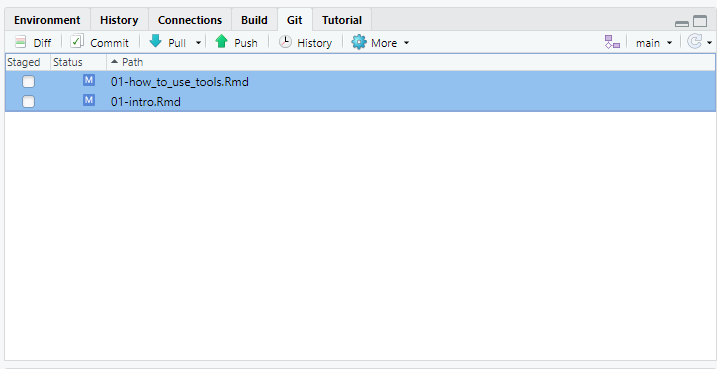
\includegraphics{01-how_to_use_tools_insertimage_1.png}

\hypertarget{tham-khux1ea3o}{%
\section{Tham khảo}\label{tham-khux1ea3o}}

\url{https://rstats.wtf/}

\hypertarget{anova-rcbd}{%
\chapter{ANOVA RCBD}\label{anova-rcbd}}

Dataset

\begin{Shaded}
\begin{Highlighting}[]
\FunctionTok{library}\NormalTok{(googlesheets4)}
\FunctionTok{gs4\_deauth}\NormalTok{()}
\NormalTok{data\_rcbd }\OtherTok{\textless{}{-}} \FunctionTok{read\_sheet}\NormalTok{(}\StringTok{\textquotesingle{}1dFmKOhpYABrPR\_e5MF27W2LSbaAGdt5dFVV3zc1H47I\textquotesingle{}}\NormalTok{)}
\end{Highlighting}
\end{Shaded}

\begin{verbatim}
## v Reading from "raw_data".
\end{verbatim}

\begin{verbatim}
## v Range 'Sheet1'.
\end{verbatim}

\begin{Shaded}
\begin{Highlighting}[]
\FunctionTok{print}\NormalTok{(data\_rcbd, }\AttributeTok{n =} \ConstantTok{Inf}\NormalTok{)}
\end{Highlighting}
\end{Shaded}

\begin{verbatim}
## # A tibble: 48 x 3
##    block  treatment yield
##    <chr>  <chr>     <dbl>
##  1 block1 TAL102     9.66
##  2 block1 TAL379     9.36
##  3 block1 TAL206     8.41
##  4 block1 TAL435     8.61
##  5 block1 TAL411     9.2 
##  6 block1 ALLEN527   8.11
##  7 block1 TAL211     8.83
##  8 block1 TAL487     6.27
##  9 block1 CB1795     6.79
## 10 block1 TAL650     6.95
## 11 block1 TAL649     6.55
## 12 block1 TAL860     6   
## 13 block1 TAL183     6.11
## 14 block1 TAL378     5.39
## 15 block1 CONTROL1   1.53
## 16 block1 CONTROL2   6.41
## 17 block2 TAL102    10.6 
## 18 block2 TAL379     9   
## 19 block2 TAL206     9.44
## 20 block2 TAL435     9.23
## 21 block2 TAL411     8.19
## 22 block2 ALLEN527   8.82
## 23 block2 TAL211     6.32
## 24 block2 TAL487     8.67
## 25 block2 CB1795     8.17
## 26 block2 TAL650     5.83
## 27 block2 TAL649     4.82
## 28 block2 TAL860     4.83
## 29 block2 TAL183     3.46
## 30 block2 TAL378     4.46
## 31 block2 CONTROL1   1.3 
## 32 block2 CONTROL2   7.83
## 33 block3 TAL102    10.8 
## 34 block3 TAL379    10.5 
## 35 block3 TAL206    10.2 
## 36 block3 TAL435     8.22
## 37 block3 TAL411     8.46
## 38 block3 ALLEN527   8.62
## 39 block3 TAL211     9.14
## 40 block3 TAL487     8.35
## 41 block3 CB1795     5.7 
## 42 block3 TAL650     6.83
## 43 block3 TAL649     8.1 
## 44 block3 TAL860     6.54
## 45 block3 TAL183     5.51
## 46 block3 TAL378     5.07
## 47 block3 CONTROL1   1.8 
## 48 block3 CONTROL2   5.83
\end{verbatim}

ANOVA

\begin{Shaded}
\begin{Highlighting}[]
\FunctionTok{library}\NormalTok{(agricolae)}
\NormalTok{outAOV }\OtherTok{\textless{}{-}} \FunctionTok{aov}\NormalTok{(yield }\SpecialCharTok{\textasciitilde{}}\NormalTok{ block }\SpecialCharTok{+}\NormalTok{ treatment, }\AttributeTok{data =}\NormalTok{ data\_rcbd)}
\NormalTok{outAOV}
\end{Highlighting}
\end{Shaded}

\begin{verbatim}
## Call:
##    aov(formula = yield ~ block + treatment, data = data_rcbd)
## 
## Terms:
##                     block treatment Residuals
## Sum of Squares    2.42538 217.47868  27.94669
## Deg. of Freedom         2        15        30
## 
## Residual standard error: 0.9651716
## Estimated effects may be unbalanced
\end{verbatim}

Check assumptions

\begin{Shaded}
\begin{Highlighting}[]
\FunctionTok{plot}\NormalTok{(}\FunctionTok{fitted}\NormalTok{(outAOV), }\FunctionTok{residuals}\NormalTok{(outAOV))}
\end{Highlighting}
\end{Shaded}

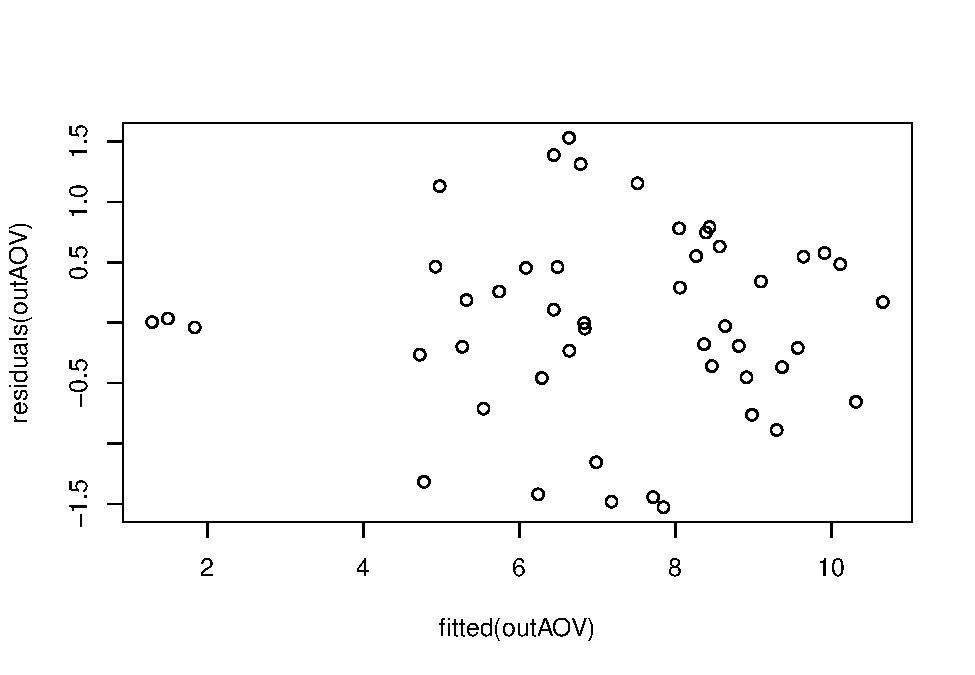
\includegraphics{_main_files/figure-latex/unnamed-chunk-5-1.pdf}

\begin{Shaded}
\begin{Highlighting}[]
\FunctionTok{hist}\NormalTok{(}\FunctionTok{residuals}\NormalTok{(outAOV))}
\FunctionTok{lines}\NormalTok{(}\FunctionTok{density}\NormalTok{(}\FunctionTok{residuals}\NormalTok{(outAOV)))}
\end{Highlighting}
\end{Shaded}

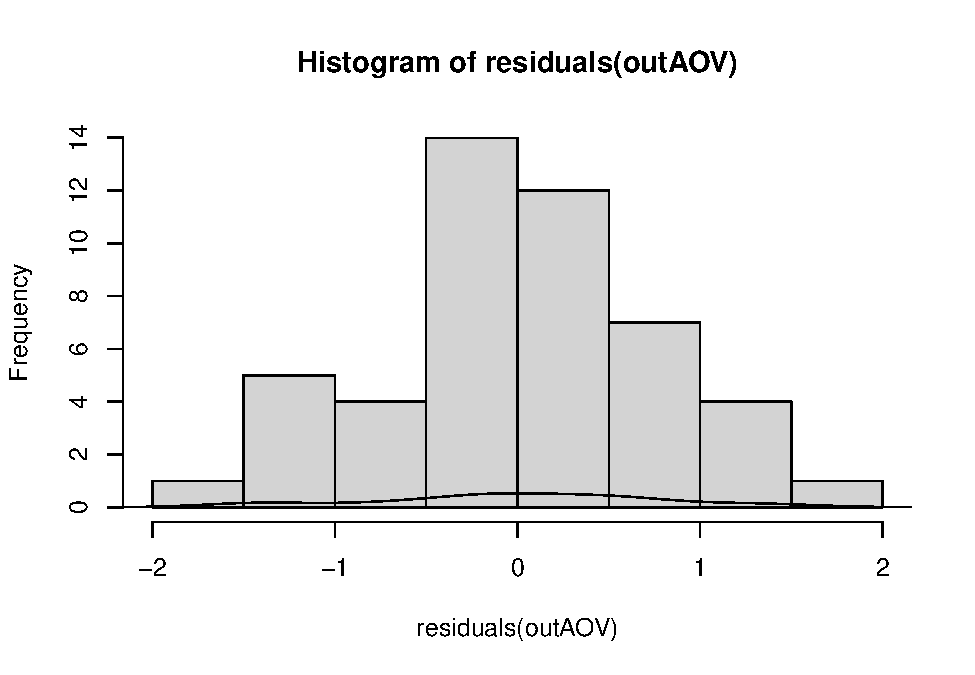
\includegraphics{_main_files/figure-latex/unnamed-chunk-5-2.pdf}

\begin{Shaded}
\begin{Highlighting}[]
\FunctionTok{hist}\NormalTok{(}\FunctionTok{residuals}\NormalTok{(outAOV), }\AttributeTok{prob =} \ConstantTok{TRUE}\NormalTok{)}
\FunctionTok{lines}\NormalTok{(}\FunctionTok{density}\NormalTok{(}\FunctionTok{residuals}\NormalTok{(outAOV)))}
\end{Highlighting}
\end{Shaded}

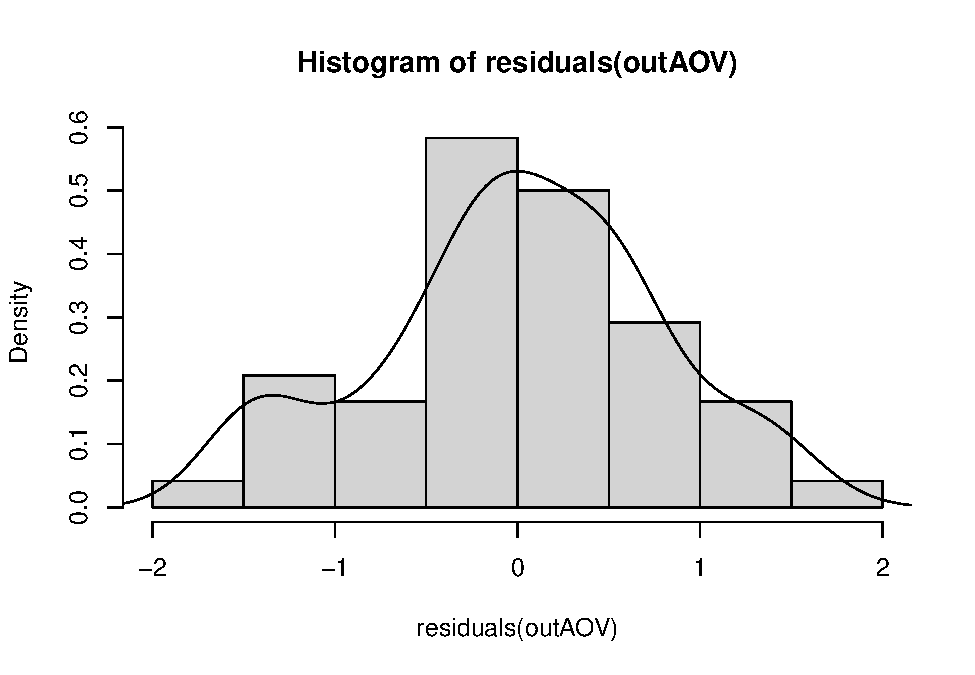
\includegraphics{_main_files/figure-latex/unnamed-chunk-5-3.pdf}

\begin{Shaded}
\begin{Highlighting}[]
\FunctionTok{library}\NormalTok{(ggpubr)}
\end{Highlighting}
\end{Shaded}

\begin{verbatim}
## Loading required package: ggplot2
\end{verbatim}

\begin{Shaded}
\begin{Highlighting}[]
\FunctionTok{ggqqplot}\NormalTok{(}\FunctionTok{residuals}\NormalTok{(outAOV))}
\end{Highlighting}
\end{Shaded}

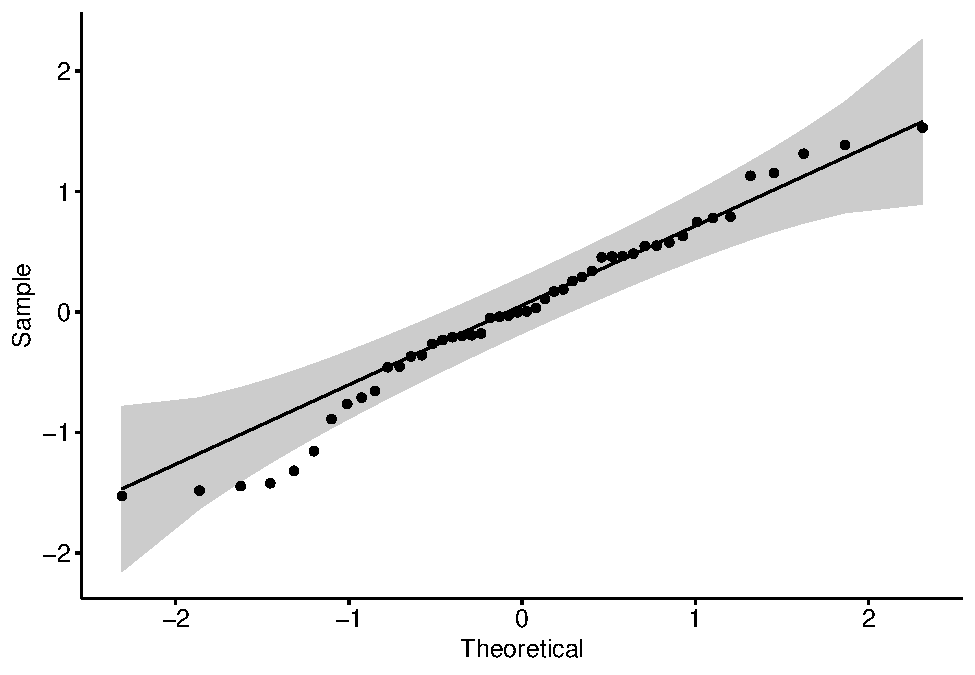
\includegraphics{_main_files/figure-latex/unnamed-chunk-5-4.pdf}

ANOVA table

\begin{Shaded}
\begin{Highlighting}[]
\FunctionTok{anova}\NormalTok{(outAOV)}
\end{Highlighting}
\end{Shaded}

\begin{verbatim}
## Analysis of Variance Table
## 
## Response: yield
##           Df  Sum Sq Mean Sq F value    Pr(>F)    
## block      2   2.425  1.2127  1.3018     0.287    
## treatment 15 217.479 14.4986 15.5638 3.284e-10 ***
## Residuals 30  27.947  0.9316                      
## ---
## Signif. codes:  0 '***' 0.001 '**' 0.01 '*' 0.05 '.' 0.1 ' ' 1
\end{verbatim}

t-test LSD

\begin{Shaded}
\begin{Highlighting}[]
\NormalTok{outFactorial }\OtherTok{\textless{}{-}}\FunctionTok{LSD.test}\NormalTok{ (outAOV, }\FunctionTok{c}\NormalTok{(}\StringTok{"treatment"}\NormalTok{), }\AttributeTok{main =} \StringTok{"yield \textasciitilde{} block + treatment"}\NormalTok{,}\AttributeTok{console=}\ConstantTok{TRUE}\NormalTok{)}
\end{Highlighting}
\end{Shaded}

\begin{verbatim}
## 
## Study: yield ~ block + treatment
## 
## LSD t Test for yield 
## 
## Mean Square Error:  0.9315563 
## 
## treatment,  means and individual ( 95 %) CI
## 
##              yield       std r       LCL       UCL  Min   Max
## ALLEN527  8.516667 0.3661056 3 7.3786265  9.654707 8.11  8.82
## CB1795    6.886667 1.2378341 3 5.7486265  8.024707 5.70  8.17
## CONTROL1  1.543333 0.2502665 3 0.4052932  2.681374 1.30  1.80
## CONTROL2  6.690000 1.0289801 3 5.5519598  7.828040 5.83  7.83
## TAL102   10.363333 0.6198656 3 9.2252932 11.501374 9.66 10.83
## TAL183    5.026667 1.3895443 3 3.8886265  6.164707 3.46  6.11
## TAL206    9.346667 0.8936629 3 8.2086265 10.484707 8.41 10.19
## TAL211    8.096667 1.5464260 3 6.9586265  9.234707 6.32  9.14
## TAL378    4.973333 0.4724757 3 3.8352932  6.111374 4.46  5.39
## TAL379    9.616667 0.7774531 3 8.4786265 10.754707 9.00 10.49
## TAL411    8.616667 0.5229085 3 7.4786265  9.754707 8.19  9.20
## TAL435    8.686667 0.5093460 3 7.5486265  9.824707 8.22  9.23
## TAL487    7.763333 1.3031245 3 6.6252932  8.901374 6.27  8.67
## TAL649    6.490000 1.6408230 3 5.3519598  7.628040 4.82  8.10
## TAL650    6.536667 0.6149255 3 5.3986265  7.674707 5.83  6.95
## TAL860    5.790000 0.8741281 3 4.6519598  6.928040 4.83  6.54
## 
## Alpha: 0.05 ; DF Error: 30
## Critical Value of t: 2.042272 
## 
## least Significant Difference: 1.609432 
## 
## Treatments with the same letter are not significantly different.
## 
##              yield groups
## TAL102   10.363333      a
## TAL379    9.616667     ab
## TAL206    9.346667    abc
## TAL435    8.686667     bc
## TAL411    8.616667     bc
## ALLEN527  8.516667     bc
## TAL211    8.096667    bcd
## TAL487    7.763333     cd
## CB1795    6.886667     de
## CONTROL2  6.690000     de
## TAL650    6.536667    def
## TAL649    6.490000    def
## TAL860    5.790000     ef
## TAL183    5.026667      f
## TAL378    4.973333      f
## CONTROL1  1.543333      g
\end{verbatim}

  \bibliography{book.bib,packages.bib}

\end{document}
